\documentclass{article}

\usepackage[english]{babel}
\usepackage[letterpaper,top=2.5cm,bottom=2.5cm,left=2.5cm,right=2.5cm,marginparwidth=1.75cm]{geometry}
\usepackage{amsmath, graphicx, tikz, pgfplots, multirow, newlfont, gensymb, indentfirst, bm, setspace, fancyhdr, pdfpages, xurl}
\pagestyle{fancy}
\fancyhf{}
\rhead{Group 2 \\ 10/26/22}
\lhead{CE-321\\Structural Engineering}
\cfoot{\thepage}
\renewcommand{\headrulewidth}{1.5pt}
\setlength{\headheight}{22.6pt}
\usepackage[colorlinks=true, allcolors=black]{hyperref}
\setlength\parindent{24pt}
\pgfplotsset{scaled y ticks=false}
\pgfplotsset{scaled x ticks=false}
\pgfplotsset{width=12cm, compat=1.18}

\begin{document}
    \begin{titlepage}
    \begin{center}
    {{\Large{\textsc{The Cooper Union for the Advancement of Science and Art}}}} \rule[0.1cm]{15.8cm}{0.1mm}
    \rule[0.5cm]{15.8cm}{0.6mm}
    {\small{\bf DEPARTMENT OF CIVIL AND ENVIRONMENTAL ENGINEERING}}\\
    {\footnotesize{STRUCTURAL ENGINEERING LABORATORY}}
    \end{center}
    \vspace{15mm}
    \begin{center}
    {\large{\bf LAB 5\\}}
    \vspace{5mm}
    {\Large{\bf COMPRESSIVE TESTING OF\\}}
    \vspace{2mm}
    {\Large{\bf STANDARD CONCRETE CYLINDER}}
    \end{center}
    \vspace{35mm}
    \par
    \noindent
    \hfill
    \vspace{20mm}
    \begin{center}
    {\large{ {\bf Group 2} \\ { Jenna Manfredi\hspace{5mm}David Madrigal\hspace{5mm}Gila Rosenzweig\\Nicole Shamayev\hspace{5mm}Jake Sigman}}}
    \vspace{40mm}
    {\large {\bf \\CE-321 \\ 12/14/22 \\}}
    \vspace{15mm}
    {\normalsize{Professor Tzavelis \\ Avery Kugler \\ Lionel Gilliar-Schoenenberger \\ Crystal Woo}}
    \end{center}
\end{titlepage}
    \doublespacing
    \tableofcontents
    \newpage
    \addcontentsline{toc}{section}{List of Tables}
    \listoftables
    \addcontentsline{toc}{section}{List of Figures}
    \listoffigures
    \newpage
    \section{Objective}
    \indent The objective of this experiment is to compare the theoretical and experimental buckling load vs slenderness ratio curves of an aluminum rod. During this experiment, 6 groups, given their own thin aluminum column, tested for the buckling load using a Tinies Olsen impact tester. The columns were pin - pin connected; when a load was applied, the columns experienced buckling along their weak axes. Testing the buckling load of a beam has significant engineering importance when considering what dimensions to use for design. Even though the buckling in this experiment was elastic, any buckling of a beam could cause significant shifts in a structure resulting in potential failures. Also, distinguishing the difference between the experimental and theoretical P critical and critical stress are vital to imposing safety factors during design. The experiment is conducted in the Civil Engineering Structures Lab at the Cooper Union (room LL220).
    \newpage
    \section{Procedure}
    \indent The materials used for this lab include an aluminum rod, a Tinius Olsen material testing device, a vernier caliper, and a tape measure. First, the width of the aluminum rod is measured using the vernier caliper to the nearest thousandth of an inch. This is useful for  calculating the cross section of the beam, which is necessary for the later critical stress calculations. Then a tape measure is used to measure the length of the aluminum rod. This would be used for the slenderness ratio values that need to be plotted in the final results.\\
    \indent After the beam measurements are taken, the aluminum rod is ready for the Tinius Olsen. A pin-pin connection is used to fasten the aluminum rod in the material testing device. After fastening the rod tight enough so there's no slack, the wheel on the Tinius Olsen is turned to load the rod with force. The beam bends along its weak axis. The technician turning the force wheel notes the increasing force values until the force dial stops. This indicates the rod is buckling since no additional force can be placed on the rod. The buckling load value is then  recorded, and used for later calculations and plots. When the rod is unloaded, the deflection springs back to place indicating an elastic deformation, and the experiment is concluded. 

    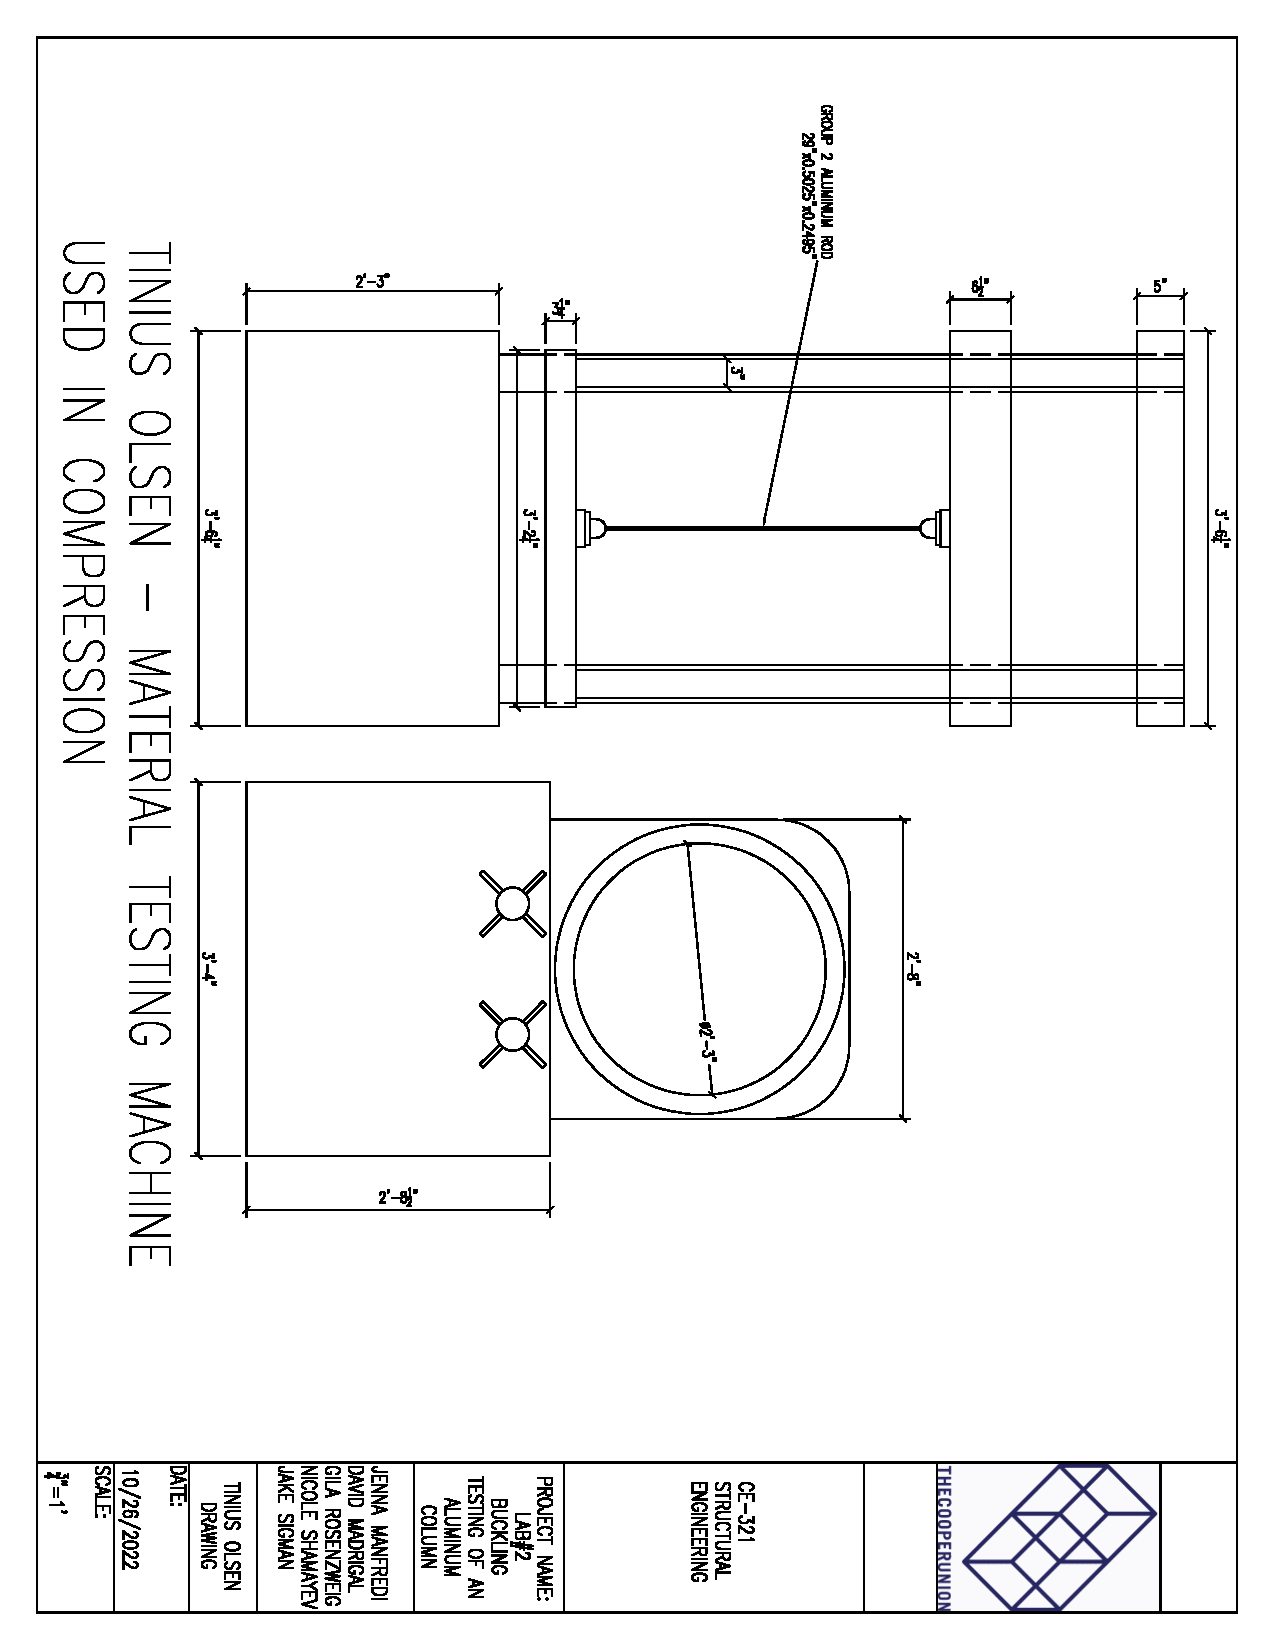
\includepdf[pages=-,pagecommand={\phantomsection\addcontentsline{toc}{subsection}{Equipment Drawing}\thispagestyle{plain}}]{dwg.pdf}
    \newpage
    \section{Theory}
    \noindent In the study of materials undergoing tensile loads, the behavior of the elastic region of the material is governed by Hooke's Law: 
    \begin{equation}
        \sigma = E \varepsilon 
    \end{equation}
    Where $\sigma$ is the applied stress, \emph{E} is the \emph{modulus of elasticity} of the material, and $\varepsilon$ is the strain. This holds true for compression loads as well; however, equation 1 fails to consider the stability of the member in question. Specifically, compression members undergo \emph{buckling}, which is the phenomenon observed as the shape change of a member. For structural engineers, this highly relevant in the design and analysis of columns, which primarily transfer compressive loads and are thus the most susceptible to buckling. A column with length \emph{L} made of a material with modulus of elasticity \emph{E} will buckle at the critical load $P_{cr}$ as governed by the following equation: 
    \begin{equation}
        P_{cr} = \frac{\pi^2 E I}{(KL)^2} 
    \end{equation}
    where $I$ is the moment of inertia of the cross section of the column, and $K$ is the \emph{effective length constant}. Equation 2 is defined as \emph{Euler's formula}. The derivation of this formula stems from considering the flexure equation defined below as bending a column laterally as opposed to a beam vertically:
    \begin{equation}
    \frac{d^2y}{dx^2} = \frac{M}{EI}
    \end{equation}
    where $M$ is the bending moment. The buckling of the column defines $M$ at a point of the column as $-Py$ where $P$ is the compressive load, and y is the offset of the column laterally. Thus, equation 3 simplifies to \[
        \frac{d^2y}{dx^2} = \frac{-Py}{EI}
    \]
    The general solution of this differential equation is 
    \[ y = A \sin px + B \cos px\]
    where \[ p^2 = \frac{P}{EI}\]
    \newpage
    \noindent The offset at the ends of a column must be equal to 0, and thus from the boundary equations,
    \[ A \sin pL = 0\]
    and $B = 0$.
    \\
    By the zero-product property, either $A$ must be equal to 0 or $\sin pL$ must be equal to 0. If $A$ is 0, this defines the column as a straight line as $y=0$. However, if $\sin pL$ is 0, it means $pL$ must be an integer multiple of $\pi$. Thus, $pL = n \pi$ where $n$ is an integer. \\
    Therefore, to solve for P, we substitute back into the flexure formula:
    \[ p^2 = \frac{n^2 \pi^2}{L^2} \Rightarrow \frac{P}{EI} = \frac{n^2 \pi^2}{L_{e}^2}\]
    The smallest value for $P$ is defined by $n = 1$, which is equivalent to equation 3, and thus the smallest load is denoted as the critical load $P_{cr}$. Here $L_{e}$ is defined as the effective length of the column and is equivalent to $kL$.\\
    Of importance now is the \emph{critical stress} $\sigma_{cr}$. Euler's formula is divided by the cross sectional area of the member $A$: 
    \[P_{cr} = \frac{\pi^2 E I}{(L_e)^2} \Rightarrow \frac{P_{cr}}{A} = \frac{\frac{\pi^2 E I}{(L_e)^2}}{A}\]
    \[\sigma_{cr} = \frac{\pi^2 E I}{(L_e)^2 A}\]
    Because $I$ is defined to be equal to $A r^2$, where $r$ is the \emph{radius of gyration}, it follows that $\frac{I}{A}$ is equal to $r^2$. Substituting,
    \[\sigma_{cr} = \frac{\pi^2 E r^2}{(L_e)^2 }\]
    Thus, the equation for critical buckling stress can be written as
    \begin{equation}
        \sigma_{cr} = \frac{\pi^2 E}{(\frac{L_e}{r})^2}
    \end{equation}
    Euler's formula assumes that bending stress caused by the moment under compressive loading is much greater than the direct axial stress; thus it was derived from the flexure formula and not from a deeper analysis of Hooke's law. However, this theory of buckling fails to account for a variety of inconsistencies; for one, Euler's theory fails to account for eccentric loading which is almost a certainty due to the impossibility of a load passing directly through the centroid of the cross-section. Additionally, failure of the column is assumed to occur only from buckling and not from yielding. However, for shorter, larger-area columns it is likely  that the column will yield before buckling as the critical stress would be greater than the yield stress. Thus, Euler's theory of buckling is a highly simplified model that only works for a certain subset of possible columns under the most ideal conditions; in practice, it is beneficial to base buckling calculations for columns of intermediate and shorter length off of empirical data and/or a combination of Euler's formula. However, for the testing of an aluminum rod with a high slenderness ratio, Euler's theory is the most efficient measure of the critical load and stress; thus, Euler's formula will be used as the primary analytical tool for this laboratory experiment. 
    \\
    While columns are the members structural engineers are most interested in, any member undergoing pure compression is susceptible to buckling; an example of this is the buckling of railroad tracks under hot weather. Similarly, the buckling of plates can be a problem for both dynamic and static engineering. Lastly, members can undergo a hybrid of torsion and buckling, known as flexural-torsional buckling, which must be accounted for in the design of the member. Thus, buckling persists as an inescapable phenomenon in structural engineering and both theoretical and empirical understanding of how members will buckle is crucial to have in an engineers repertoire. 
    
    \newpage
    {\singlespacing\section{Sample Calculations}
    \subsection{Moment of Inertia}
    \[I = \frac{1}{12}\times b\times h^3\]
    \[I = \frac{1}{12}\times 0.5025\text{ in}\times 0.2495\text{ in}^3 = \boxed{6.503\times 10^{-4} \text{ in}^4}\] 
    \subsection{Cross-Sectional Area}
    \[A=b\times h\]
    \[A=0.5025\text{ in}\times 0.2495\text{ in}=\boxed{0.1254\text{ in}^2}\]
    \subsection{Critical Buckling Load}
    \[P_\text{cr} = \frac{\pi^2\times E\times I}{L^2}\]
    \[P_\text{cr} = \frac{\pi^2(10000\text{ ksi})(6.503\times 10^{-4}\text{in}^4)}{(29 \text{ in})^2} = \boxed{76.33 \text{ lbs}}\]
    \subsection{Critical Stress}
    \[\sigma_\text{cr} = \frac{P_\text{cr}}{A}\]
    \[\sigma_\text{cr} = \frac{73\text{ lbs}}{0.1254\text{ in}^2}= \boxed{582.26\text{ psi}}\]
    \subsection{Radius of Gyration}
    \[r=\sqrt{\frac{I}{A}}\]
    \[r=\sqrt{\frac{6.503\times 10^{-4}\text{ in}^4}{0.1254\text{ in}^2}}=\boxed{0.0720\text{ in}}\]
    \subsection{Slenderness Ratio}
    \[\text{Slenderness Ratio} = \frac{L}{r}\]
    \[\text{Slenderness Ratio}  = \frac{29\text{ in}}{0.0720\text{ in}}=\boxed{402.64}\]
    \subsection{Error}
    \[\%_\text{Error}=\frac{|\text{Theoretical}-\text{Experimental}|}{\text{Theoretical}}\times 100\%\]
    \[\%_\text{Error} = \frac{|608.78-582.26|}{608.78}\times 100 = \boxed{4.26\%} \] 
    }\newpage
    \section{Results}
    \begin{center}
        \doublespacing
    \addcontentsline{lot}{table}{Table 1: Measured Data}
    {\large{\bf Table 1: Measured Data\\}}
    \vspace{3mm}
    \begin{tabular}{|c c c c|}
        \hline
        \textbf{Group} & \textbf{Length (in)} & \textbf{Base (in)} & \textbf{Thickness (in)} \\\hline
        1  & 35      & 0.502        & 0.2525      \\
        2  & 29      & 0.5025       & 0.2495      \\
        3  & 25      & 0.5          & 0.25        \\
        4  & 27      & 0.5          & 0.25        \\
        5  & 29.9375 & \multicolumn{2}{c|}{Diameter = 0.3735}  \\
        6  & 30.5625 & 0.5          & 0.5        \\\hline
    \end{tabular}
    \vspace{6mm}
    \addcontentsline{lot}{table}{Table 2: Calculated Data}
    {\large{\bf \\Table 2: Calculated Data\\}}
    \vspace{3mm}
    \begin{tabular}{|c c c c|}
        \hline
        \(\bm{A}\) (\(\textbf{in}^{\bm{2}}\)) & \(\bm{I}\) (\(\textbf{in}^{\bm{4}}\)) & \(\bm{r}\) \textbf{(in)} & \(\bm{\frac{L}{r}}\) \\\hline
        0.13 & 0.0007 & 0.07 & 480.17 \\
        0.13 & 0.0007 & 0.07 & 402.64 \\
        0.13 & 0.0007 & 0.07 & 346.41 \\
        0.13 & 0.0007 & 0.07 & 374.12 \\
        0.11 & 0.0010 & 0.09 & 320.62 \\
        0.25 & 0.0052 & 0.14 & 211.74 \\\hline
    \end{tabular}
    \vspace{6mm}
    \addcontentsline{lot}{table}{Table 3: Experimental Data}
    {\large{\bf \\Table 3: Experimental Data\\}}
    \vspace{3mm}
    \begin{tabular}{|c c c|}
        \hline
        \textbf{Group} & \textbf{\(\textbf{P}_\textbf{cr}\) (lbs)} & \textbf{\(\bm{\sigma}_\textbf{cr}\) (psi)}  \\\hline
        1     & 55    & 433.91  \\
        2     & 73    & 582.26  \\
        3     & 95    & 760.00  \\
        4     & 85    & 680.00  \\
        5     & 100   & 912.70  \\
        6     & 461   & 1844.00 \\\hline
    \end{tabular}
    \vspace{6mm}
    \newpage
    \addcontentsline{lot}{table}{Table 4: Theoretical Data}
    {\large{\bf Table 4: Theoretical Data\\}}
    \vspace{3mm}
    \begin{tabular}{|c c c|}
        \hline
        \textbf{Group} & \textbf{\(\textbf{P}_\textbf{cr}\) (lbs)} & \textbf{\(\bm{\sigma}_\textbf{cr}\) (psi)}  \\\hline
        1     & 54.26  & 428.06  \\
        2     & 76.33  & 608.78  \\
        3     & 102.81 & 822.47  \\
        4     & 88.14  & 705.13  \\
        5     & 105.20 & 960.13  \\
        6     & 550.33 & 2201.31 \\\hline
    \end{tabular}
    \end{center}
    \begin{center}
        \doublespacing
            \begin{tikzpicture}[baseline=(current bounding box.center)]
                \addcontentsline{lof}{figure}{Figure 1: Stress vs. Slenderness Ratio}
                \begin{axis}[
                    title={\textbf{Figure 1: Stress vs. Slenderness Ratio}},
                    xlabel={\(\frac{L}{r}\)},
                    ylabel={\(\sigma_\text{cr}\) (psi)},
                    ymin=0, ymax=2500,
                    xmin=0, xmax=600,
                    xticklabel style={
                    /pgf/number format/precision=3,
                    /pgf/number format/fixed},
                    ytick={0,500,1000,1500,2000,2500},
                    xtick={0,100,200,300,400,500,600},
                    ymajorgrids=true,
                    grid style=dashed,
                    cells={anchor=west},
                    legend cell align={left},
                    width=0.9\textwidth,
                    height=1.3\textwidth
                ]
                
                \addplot[only marks, red] table [x=t_lr, y=t_stress] {1.csv};
                \addplot[only marks, blue] table [x=t_lr, y=e_stress] {1.csv};
                \addplot[smooth, dashed, blue] table [x=x, y=y] {trend1.csv};
                \addplot[smooth, dashed, red] table [x=x, y=y] {trend2.csv};
                \addlegendentry{Experimental}
                \addlegendentry{Theoretical}
                \end{axis}
            \end{tikzpicture}
    \end{center}
    \newpage
    \begin{center}
        {\bf Figure 2: Aluminum Rod at Yield Force for Buckling}
        \vspace{3mm}
        \addcontentsline{lof}{figure}{Figure 2: Aluminum Rod at Yield Force for Buckling}
        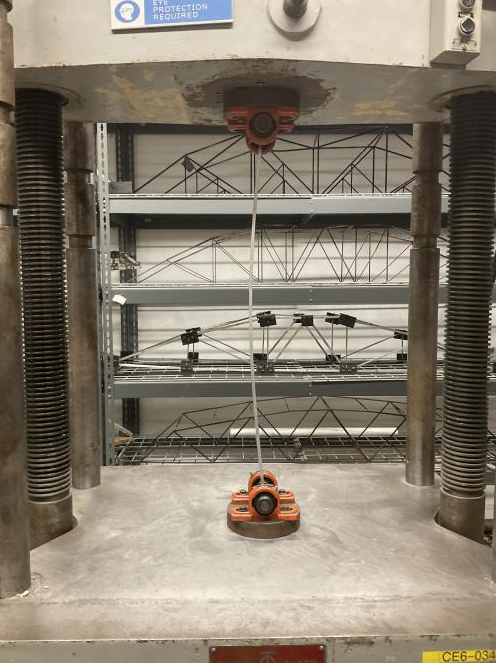
\includegraphics[scale=0.7]{pic2.png}
    \end{center}
    \newpage
    \section{Conclusion}
    \indent The objective of every engineer is to design cost-effectively, and economically; to that end, effective column design involves comparing different column design criteria and materials. Most often, carbon and low-alloy steels, stainless steels, and aluminum alloys are considered. Aluminum alloys have the ability to function effectively in many atmospheres, although they are not commonly used in structures, due to factors such as high material cost, low value of modulus of elasticity, and unfamiliarity with design methodology. Typically, steel is the material of choice for metal columns.\\
    \indent In column design, it is necessary to consider the load to which a column will be subjected and determine if the critical buckling load is below this value. Buckling is a structural instability that is associated with high compression loads resulting in a failure of a long and slender structural element (usually vertical). The failure is a lateral deformation of the element making it asymmetric at the point of deformation with respect to its central axis. Failure is most often in the column axis with the smallest moment of inertia and radius of gyration.  \\
    \indent Compressive strengths of a material, in much the same way that tensile strengths are variable, are affected by several variables: allow composition, temperature, geometry of the specimen, and test conditions. There are experiments which test the effect high temperatures can have on the buckling strength of a column and the extent to which Euler’s theorem holds true for columns in such conditions, studies which compare the effects of alloying and casting conditions. This laboratory experiment tested small aluminum columns of known dimensions to visually magnify buckling behavior; their buckling load is observed in the Tinius Olsen testing machine and compared with the theoretical critical loading value. Specimens were placed between two pinned ends and subjected to loading until buckling was no longer increasing noticeably. Using Euler’s buckling equation, the specimens have an effective length factor of 1.0, as the ends are rotationally free and translationally fixed. Six aluminum members were tested, with experimental critical load values of 55, 73, 95, 85, 100, and 461 lbs. Using this data, the critical load stress was calculated for each member, and found to be 433.9, 582.3, 760.0, 680.0, 912.7, and 1844 psi. Observationally, all specimens buckled on the weak axis, as was expected. The curve was expectedly like that of the theoretical pinned-pinned connection, with the curve being continuous from each end of the column. \\
    \indent Both experimental critical load and critical load stress were compared with the theoretical values for the same properties. The largest error values were seen for specimen 6, a square section that has a larger cross-sectional area than the other five specimens, and thus saw larger theoretical and experimental value; for specimen 6, error was 16.23\%. Most specimens carry an error of less than 5\%, apart from specimen 3 and specimen 6. Average error across all specimens was 6.34\%; if specimen 6 is neglected due to its large error, percent error is reduced to 4.36\%. \\
    \indent In five of six cases, the experimental buckling load was smaller than the theoretical; such error can be due to incorrect readings of the calipers and/or measures used to determine the dimensions of the specimens, which would then inflate the theoretical critical load. Instrumental error can also play a role in the discrepancies between the values, without attributing the difference to incorrect readings; further precision may have helped get more precise dimensions, which would in turn impact the cross-sectional area, length, and calculation for critical load. Error is also possibly introduced in reading the loading on the testing machine; there can be instrumental as well as human error, with instrumental error arising from the fact that the machine is not precise to any decimal points, as were the calculated values, and human error arising from potential misreading of the load dial. Error may be introduced in calculations, if values are rounded before the final calculations; additionally, instrumental errors propagate into calculations, a possible example of which can be dimensions, which are used to calculate area, which is in turn used to calculate moment of inertia, then subsequently used to calculate the radius of gyration. The potential for rounding to occur at any point along the way means that end calculation results may be a bit different than values determined experimentally. It is further possible that the testing environment faced an elevated temperature, which can affect the behavior of the material.  \\
    \indent A limit of the experiment design is that specimens were loaded only until observational buckling stopped; it is possible that observational buckling is variable from person to person, and were another person to be conducting the test, loading might have been stopped at a higher value. To improve this experiment, it might be worthwhile to set up a reference for buckling motion that is more easily compared to than the objects in the distance; one example may be setting a closer background to the testing area against which deflection and buckling motion may be more easily detected.  \\
    \indent As seen in this experiment with the majority of specimens tested, it is not all that uncommon for a column to buckle before the theoretical critical load point. This can be due to any number of reasons or conditions, which include calculated error, elevated temperatures affecting the ductility or rigidity of a material, or the possibility for material inconsistencies (elevated potential for such inconsistencies in smaller specimens). For this reason, engineers design with consideration to a safety factor. For buckling scenarios, this may be in using an effective length factor higher than the theoretical effective length factor, as seen in the following diagram:\\

    \begin{center}
    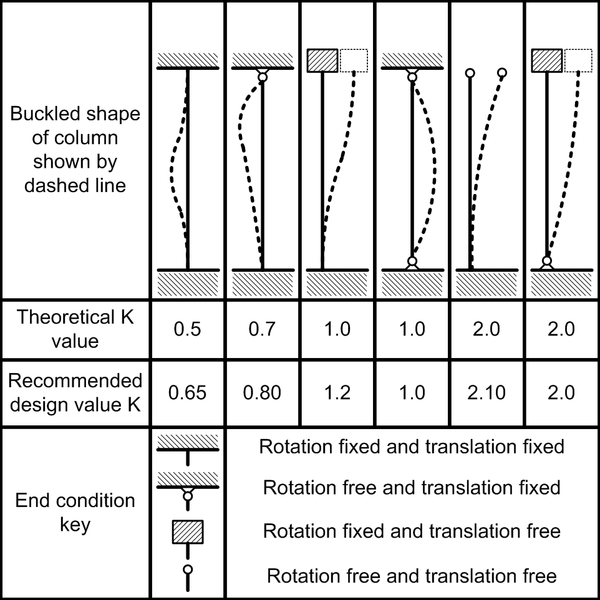
\includegraphics[scale=0.3]{pic.png}
    \end{center}

    \indent An engineers goal is to design safely, economically, and effectively: to that end, the column of smallest area feasibly for safely attaining the intended load bearing capacity should be used. This experiment provided a good visual for buckling behavior to enhance the understanding of    material behavior and how it can influence choices in engineering design.
    \newpage
    \section{References}
    
    \begin{description}
        \item Ferdinand B. \emph{et. al.} (2015). \emph{Mechanics of Materials}, 7th Ed., McGraw Hill, New York.
        \item Madeh H. Euler's Theory of Column Buckling, \url{https://theconstructor.org/structural-engg/euler-theory-column-buckling/37341/} (accessed 23 October 2022).
        \item Shaymaa, M. \emph{et. al.} (1973). Buckling at Elevated Temperature for (6061-T6) Aluminum Alloy Columns under Increasing Load, \url{https://iopscience.iop.org/article/10.1088/1742-6596/1973/1/012106/pdf} (accessed 23 October 2022).
        \item Etienne, V. (1998). The Flexural Buckling Strength of Aluminum Columns, \url{https://core.ac.uk/download/pdf/18219883.pdf} (accessed 23 October 2022).
    \end{description}
    \newpage
    \section{Appendix}
    \begin{center}
        \doublespacing
    \begin{tabular}{|c|c|c|c|c|c|c|}
        \hline
            \textbf{Group} & \textbf{1} & \textbf{2} & \textbf{3}& \textbf{4} & \textbf{5} & \textbf{6} \\ \hline
            \textbf{Width, b (in)} & 0.502 & 0.5025 & 0.5 & 0.5 & 0.3735 & 0.5 \\ \hline
            \textbf{Length, h (in)} & 0.2525 & 0.2495 & 0.25 & 0.25 & 0.3735 & 0.5 \\ \hline
            \textbf{Height, L (in)} & 35 & 29 & 25 & 27 & 29.94 & 30.56 \\ \hline
            \textbf{Cross Sectional Area, A} \textbf{(\(\textbf{in}^{\bm{2}}\))} & 0.1268 & 0.1253 & 0.125 & 0.125 & 0.1096 & 0.25 \\ \hline
            \textbf{Moment of Inertia, I (\(\textbf{in}^{\bm{4}}\))} & 0.0007 & 0.0007 & 0.0007 & 0.0007 & 0.001 & 0.0052 \\ \hline
            \textbf{Radius of Gyration, \(\bm{r}\) (in)} & 0.0729 & 0.0720 & 0.0722 & 0.0722 & 0.0934 & 0.1443 \\ \hline
            \textbf{Slenderness Ratio, \(\bm{\frac{L}{r}}\)} & 480.17 & 402.64 & 346.41 & 374.12 & 320.62 & 211.74 \\ \hline
            \textbf{Theoretical Buckling Load, \textbf{\(\textbf{P}_\textbf{cr}\) (lb)}} & 54.26 & 76.33 & 102.81 & 88.14 & 105.20 & 550.33 \\ \hline
            \textbf{Experimental Buckling Load, \textbf{\(\textbf{P}_\textbf{cr}\) (lb)}} & 55 & 73 & 95 & 85 & 100 & 461 \\ \hline
            \textbf{Theoretical Buckling Stress,  \(\bm{\sigma}_\textbf{cr}\) (psi)} & 418.06 & 608.78 & 822.47 & 705.13 & 960.13 & 2201.31 \\ \hline 
            \textbf{Experimental Buckling Stress,  \(\bm{\sigma}_\textbf{cr}\) (psi)} & 433.91 & 582.26 & 760.00 & 680.00 & 912.70 & 1844.00 \\ \hline
            \textbf{Buckling Stress Percentage Error (\%)} & 1.37 & 4.36 &7.60 & 3.56 & 4.94 & 16.26 \\\hline
        \end{tabular}
    \end{center}
\end{document}